\documentclass[10pt]{article}
\usepackage[polish]{babel}
\usepackage[utf8]{inputenc}
\usepackage[T1]{fontenc}
\usepackage{amsmath}
\usepackage{amsfonts}
\usepackage{amssymb}
\usepackage[version=4]{mhchem}
\usepackage{stmaryrd}
\usepackage{graphicx}
\usepackage[export]{adjustbox}
\graphicspath{ {./images/} }

\title{LIGA MATEMATYCZNA \\
 im. Zdzisława Matuskiego \\
 LISTOPAD 2022 \\
 SZKOŁA PODSTAWOWA \\
 klasy IV - VI }

\author{}
\date{}


\begin{document}
\maketitle
\section*{ZADANIE 1.}
Pewien bogaty logik zostawił swoim dzieciom następujący testament:\\
„W ogrodzie rosną kolejno posadzone cztery drzewa owocowe: 1 - czereśnia, 2 - grusza, 3 - jabłoń, 4 - śliwa. Pod jednym z nich zakopałem skarb. Aby go znaleźć musicie zrywać po jednym liściu z tych drzew w następujący sposób:

\[
12343211234321 \ldots
\]

Pod drzewem, z którego zerwiecie 2022 liść znajduje się skarb."\\
Które to drzewo?

\section*{ZADANIE 2.}
Figura przedstawiona na rysunku składa się z czterech przystających prostokątów. Każdy prostokąt ma boki o długości \(a\) i \(2 a\). Oblicz pole figury, jeżeli jej obwód jest równy 80 .\\
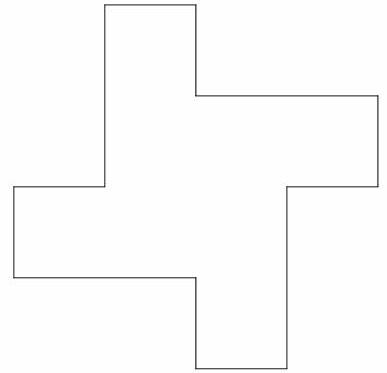
\includegraphics[max width=\textwidth, center]{2024_11_21_80308583ef159bc82e17g-1}

\section*{ZADANIE 3.}
Zagadkowy kalkulator ma tylko dwa klawisze \(+1 \mathrm{i} \times 2\). Naciśnięcie klawisza +1 powoduje dodanie 1 do liczby na wyświetlaczu, naciśnięcie klawisza \(\times 2\) powoduje pomnożenie tej liczby przez 2. Na wyświetlaczu jest teraz 0 . Czy uzyskamy liczbę 22, jeżeli klawisze można nacisnąć tylko siedem razy?

\section*{ZADANIE 4.}
Znajdź wszystkie liczby trzycyfrowe, których suma cyfr jest równa 6.

\section*{ZADANIE 5.}
Bartek wykonał dwadzieścia rzutów sześcienną kostką do gry i otrzymał w sumie 100 oczek. Co najwyżej ile razy mógł wyrzucić jedno oczko?


\end{document}